Principal component analysis (PCA) and factor analysis (FA) originated independently by Pearson in 1901 and Spearman in 1904 \cite{1901pearson, 1904spearman}. Pearson gave the first formal treatment of it not to compute principal components, but to give a new measure of what a ``best fit'' line means. On the other hand, Spearman---frustrated by the lack of rigorous analyses on nontrivial in  psychology---attempted to model the correlation between mental aptitude and sensory tasks. Though their discoveries were independent, the similarity of their models had inevitably caused their developments to coincide. 

Note that PCA is similar to linear regression in that it fits some line (or hyperplane) of best fit to some data. However, linear regression---as a model that tries to use the covariates $x$ to predict the response $y$---attempts to minimize the \textit{residual} $(y - \hat{y})^2$. If we were to flip the model and try to predict $x$ with $y$, then the best fit line would not be the same. As Pearson puts it, \textit{the most probable stature of a man with a given length of leg $l$ being $s$, the most probable length of a leg for a man of stature $s$ will not be $l$} \cite{1901pearson}. This is further motivated by the fact that in many data collecting procedures, you do not collect a perfect measurement of $x$ first and then a noisy measurement of $y$. Rather, you are usually collecting both $x$ and $y$ together at the same time, in which they may both be perceptive to error. 

\begin{figure}[H]
  \centering
  \begin{subfigure}[b]{0.4\textwidth}
  \centering
  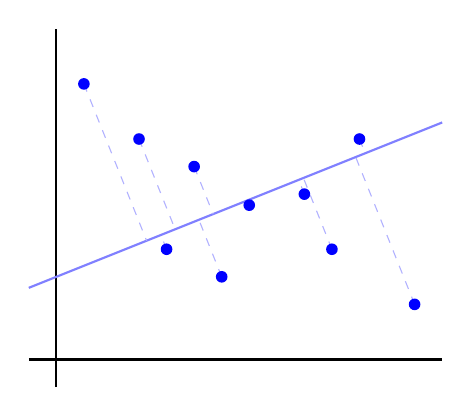
\begin{tikzpicture}[scale=0.7]
    % Draw axes
    \draw[black, line width=0.8pt] (-0.5,0) -- (7,0);
    \draw[black, line width=0.8pt] (0,-0.5) -- (0,6);
    
    % Define trend line coordinates (y = mx + b)
    \def\m{0.4}  % slope
    \def\b{1.5}  % y-intercept
    \draw[blue!50, line width=0.8pt] (-0.5,{-0.5*\m + \b}) -- (7,{7*\m + \b});
    
    % Calculate perpendicular direction vector (-m, 1) normalized
    \def\dx{-\m/sqrt(1+\m*\m)}
    \def\dy{1/sqrt(1+\m*\m)}
    
    % Points and their perpendicular projections
    % For point (x,y), intersection with line is:
    % x' = (x + m*y - m*b)/(1 + m^2)
    % y' = m*x' + b
    
    % Define and draw points with their projections
    \foreach \x/\y in {
      0.5/5,    % p1
      1.5/4,    % p2
      2/2,      % p3
      2.5/3.5,  % p4
      3/1.5,    % p5
      3.5/2.8,  % p6
      4.5/3,    % p7
      5/2,      % p8
      5.5/4,    % p9
      6.5/1     % p10
    } {
      % Calculate projection point
      \pgfmathsetmacro{\px}{(\x + \m*\y - \m*\b)/(1 + \m*\m)}
      \pgfmathsetmacro{\py}{\m*\px + \b}
      
      % Draw dashed line and point
      \draw[dashed, blue!30] (\x,\y) -- (\px,\py);
      \fill[blue] (\x,\y) circle (3pt);
    }
  \end{tikzpicture}
    \caption{PCA minimizes the orthogonal distance to the subspace. }
  \end{subfigure}
  \begin{subfigure}[b]{0.4\textwidth}
  \centering
  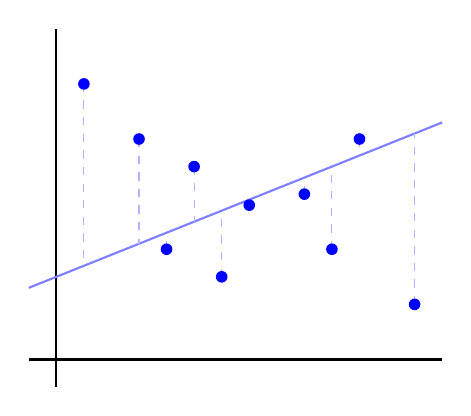
\begin{tikzpicture}[scale=0.7]
    % Draw axes
    \draw[black, line width=0.8pt] (-0.5,0) -- (7,0);
    \draw[black, line width=0.8pt] (0,-0.5) -- (0,6);
    
    % Define trend line function: y = 0.4x + 1.5
    \draw[blue!50, line width=0.8pt] (-0.5,1.3) -- (7,4.3);
    
    % Points with their actual trend line intersections
    \coordinate (p1) at (0.5,5);
    \path (0.5,1.7) coordinate (t1);  % trend point
    
    \coordinate (p2) at (1.5,4);
    \path (1.5,2.1) coordinate (t2);
    
    \coordinate (p3) at (2,2);
    \path (2,2.3) coordinate (t3);
    
    \coordinate (p4) at (2.5,3.5);
    \path (2.5,2.5) coordinate (t4);
    
    \coordinate (p5) at (3,1.5);
    \path (3,2.7) coordinate (t5);
    
    \coordinate (p6) at (3.5,2.8);
    \path (3.5,2.9) coordinate (t6);
    
    \coordinate (p7) at (4.5,3);
    \path (4.5,3.3) coordinate (t7);
    
    \coordinate (p8) at (5,2);
    \path (5,3.5) coordinate (t8);
    
    \coordinate (p9) at (5.5,4);
    \path (5.5,3.7) coordinate (t9);
    
    \coordinate (p10) at (6.5,1);
    \path (6.5,4.1) coordinate (t10);
    
    % Draw dashed lines from points to their trend line intersections
    \foreach \i in {1,...,10} {
      \draw[dashed, blue!30] (p\i) -- (t\i);
      \fill[blue] (p\i) circle (3pt);
    }
  \end{tikzpicture}
    \caption{Linear regression minimizes the residual distance to the subspace.} 
  \end{subfigure}
  \caption{Note that this is in fact different from linear regression as it minimizes the expected \textit{orthogonal distance} to the subspace, rather than the residual distance to the subspace as in linear regression.}
  \label{fig:pca_lin_reg}
\end{figure}

